%%%%%%%%%%%%%%%%%%%%%%%%%%%%%%%%%%%%%%%%%
% Jacobs Landscape Poster
% LaTeX Template
% Version 1.0 (29/03/13)
%
% Created by:
% Computational Physics and Biophysics Group, Jacobs University
% https://teamwork.jacobs-university.de:8443/confluence/display/CoPandBiG/LaTeX+Poster
% 
% Further modified by:
% Nathaniel Johnston (nathaniel@njohnston.ca)
%
% This template has been downloaded from:
% http://www.LaTeXTemplates.com
%
% License:
% CC BY-NC-SA 3.0 (http://creativecommons.org/licenses/by-nc-sa/3.0/)
%
%%%%%%%%%%%%%%%%%%%%%%%%%%%%%%%%%%%%%%%%%

%----------------------------------------------------------------------------------------
%	PACKAGES AND OTHER DOCUMENT CONFIGURATIONS
%----------------------------------------------------------------------------------------

\documentclass[final]{beamer}

\usepackage[scale=1.24]{beamerposter} % Use the beamerposter package for laying out the poster

\usetheme{confposter} % Use the confposter theme supplied with this template

\setbeamercolor{block title}{fg=ngreen,bg=white} % Colors of the block titles
\setbeamercolor{block body}{fg=black,bg=white} % Colors of the body of blocks
\setbeamercolor{block alerted title}{fg=white,bg=dblue!70} % Colors of the highlighted block titles
\setbeamercolor{block alerted body}{fg=black,bg=dblue!10} % Colors of the body of highlighted blocks
% Many more colors are available for use in beamerthemeconfposter.sty

%-----------------------------------------------------------
% Define the column widths and overall poster size
% To set effective sepwid, onecolwid and twocolwid values, first choose how many columns you want and how much separation you want between columns
% In this template, the separation width chosen is 0.024 of the paper width and a 4-column layout
% onecolwid should therefore be (1-(# of columns+1)*sepwid)/# of columns e.g. (1-(4+1)*0.024)/4 = 0.22
% Set twocolwid to be (2*onecolwid)+sepwid = 0.464
% Set threecolwid to be (3*onecolwid)+2*sepwid = 0.708

\newlength{\sepwid}
\newlength{\onecolwid}
\newlength{\twocolwid}
\newlength{\threecolwid}
\setlength{\paperwidth}{48in} % A0 width: 46.8in
\setlength{\paperheight}{37in} % A0 height: 33.1in
\setlength{\sepwid}{0.024\paperwidth} % Separation width (white space) between columns
\setlength{\onecolwid}{0.22\paperwidth} % Width of one column
\setlength{\twocolwid}{0.464\paperwidth} % Width of two columns
\setlength{\threecolwid}{0.708\paperwidth} % Width of three columns
\setlength{\topmargin}{-0.5in} % Reduce the top margin size
%-----------------------------------------------------------
\usepackage{tikz}
\usepackage{graphicx}  % Required for including images

\usepackage{booktabs} % Top and bottom rules for tables

%----------------------------------------------------------------------------------------
%	TITLE SECTION 
%----------------------------------------------------------------------------------------
\title{\textbf{QNX Realtime Operating System and Applications}}

\author{Gokul Nair (2018120039)\ , Kaustubh Venkatesh (2018120033)}

\institute{ Mentor: Prof. Anand Mane\\Embedded Systems and RTOS \\
            \ Department of Electronics and Telecommunication, Sardar Patel Institute of Technology}
\titlegraphic{
\includegraphics[width=0.08\textwidth]{spit.png}}

\begin{document}

\addtobeamertemplate{block end}{}{\vspace*{2ex}} % White space under blocks
\addtobeamertemplate{block alerted end}{}{\vspace*{2ex}} % White space under highlighted (alert) blocks

\setlength{\belowcaptionskip}{2ex} % White space under figures
\setlength\belowdisplayshortskip{2ex} % White space under equations

\begin{frame}[t] % The whole poster is enclosed in one beamer frame

\begin{columns}[t] % The whole poster consists of three major columns, the second of which is split into two columns twice - the [t] option aligns each column's content to the top

\begin{column}{\sepwid}\end{column} % Empty spacer column

\begin{column}{\onecolwid} % The first column

\begin{block}{Abstract}

Real-time operating systems (RTOS) are operating systems intended to serve time sensitive applications that process data without buffer delays. QNX is an RTOS that provides a processor distributed real-time environment based on a microkernel architecture that delivers the full device level performance of the underlying hardware. This study presents an architectural overview of QNX and its applications.

\end{block}

\vspace{10mm}
\vfill

\begin{center}

\includegraphics[width=0.6\linewidth]{qnxlogo.png}
\\*
\caption{Fig. 1 : QNX Logo}
\end{center}

\begin{block}{Introduction}
         
         QNX is a commercial Unix-like hard real-time operating system used in embedded systems.
Closed-source OS which was developed in the 1980s and was acquired by Blackberry in 2010.
Based on a microkernel RTOS based architecture. Also includes a embeddable Graphical User Interface (GUI).
\vspace{10mm}
\vfill
   \begin{center}
 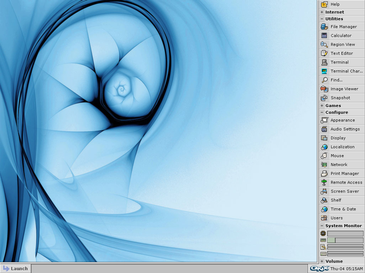
\includegraphics[width=17cm]{QNX_6.4.1_screenshot.png}
 \\
 \\
 \caption{Fig. 2 :  QNX GUI Window}
        \end{center}
\vspace{5mm}
\vfill
One of the first widespread uses of the QNX real-time OS (RTOS) was in the non-embedded world when it was selected as the operating system for the Ontario education system's own computer design, the Unisys ICON. Over the years QNX was used mostly for larger projects, as its 44k kernel was too large to fit inside the one-chip computers of the era. 
    
\end{block}
\end{column} % End of the first column

\begin{column}{\sepwid}\end{column} % Empty spacer column

\begin{column}{\twocolwid} % Begin a column which is two columns wide (column 2)

\begin{columns}[t,totalwidth=\twocolwid] % Split up the two columns wide column

\begin{column}{\onecolwid}\vspace{-.6in} % The first column within column 2 (column 2.1)

%----------------------------------------------------------------------------------------
%	MATERIALS
%----------------------------------------------------------------------------------------

\begin{block}{Features}
\begin{enumerate}
\item Multi-platform OS which can run on x86-64, ARM32 and ARM64.
\item The QNX kernel ‘procnto’ contains CPU scheduling, interprocess communication, interrupt redirection and timers.
\item Kernel runs in the form of a number of small tasks. A special process ‘proc’ performs process creation and memory management.
\item Supports symmetric multiprocessing, processor affinity, strict priority-preemptive scheduling and adaptive partition scheduling (APS).
\end{enumerate}
\vspace{10mm}
\vfill
\begin{center}
 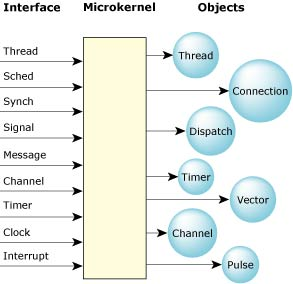
\includegraphics[width=18cm]{qnx_kernel.jpg}\\
  \caption{Fig. 3 : QNX Microkernel}
\end{center}

\end{block}


\begin{block}{Memory Management}
\begin{enumerate}
    \item By design, QNX's architecture helps ensure that faults, including memory errors, are confined to the program that caused them. Programs are less likely to cause a cascade of faults because processes are isolated from each other and from the microkernel. 
    \item Even device drivers behave like regular debuggable processes. This robust architecture ensures that crashing one program has little or no effect on other programs throughout the system. If a program faults, the system can be sure that the error is restricted to that process's operation. 
\end{enumerate}

\end{block}


\end{column} % End of column 2.1

\begin{column}{\onecolwid}\vspace{-.6in} % The second column within column 2 (column 2.2)

\begin{block}{Applications}

\begin{enumerate}
\item Used in automobile infotainment systems. 
\item Used in Blackberry tablets and smartphones.
\end{enumerate}

\vspace{10mm}
\vfill

\begin{center}
 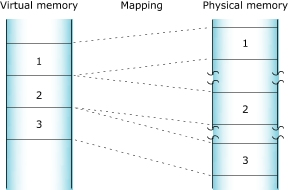
\includegraphics[width=20cm]{qnx_memory.jpg}\\
 \caption{Fig. 4 : Memory Management in QNX}
\end{center}

\end{block}

\begin{block}{Architecture}
    \begin{enumerate}
\item Inter-process communication is done using the MsgSend operation, a subroutine-call like operation. Handled based on thread priority.
\item The boot loader can load an image containing the kernel and any desired set of user programs and shared libraries. There are no device drivers in the kernel.

\item QNX's full memory protection means that almost all the memory addresses a program encounters are virtual addresses. The process manager maps the program's virtual memory addresses to the actual physical memory.
\end{enumerate}

\vspace{10mm}
\vfill

\begin{center}
 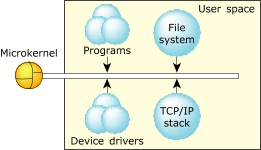
\includegraphics[width=23cm]{qnx_mem.jpg}
 \vspace{5mm}
\vfill
 \caption{Fig. 5 : Memory Interfacing in QNX}
\end{center}

\end{block}

\end{column} % End of column 2.1

\end{columns} % End of the split of column 2

\end{column} % End of the second column

\begin{column}{\sepwid}\end{column} % Empty spacer column

\begin{column}{\onecolwid} % The third column

\begin{block}{Conclusion}
\begin{enumerate}
    \item RTOS are essential in systems where proper temporal execution of processes is imperative such as military, medical and automobile applications.
    \item QNX is one of the most widely used RTOS systems owned by Blackberry. It uses a microkernel based architecture and also includes a GUI for systems with displays.
    \item It uses MsgSnd operations to perform inter-process communications and memory management is done using virtualization.
\end{enumerate}

\begin{center}
 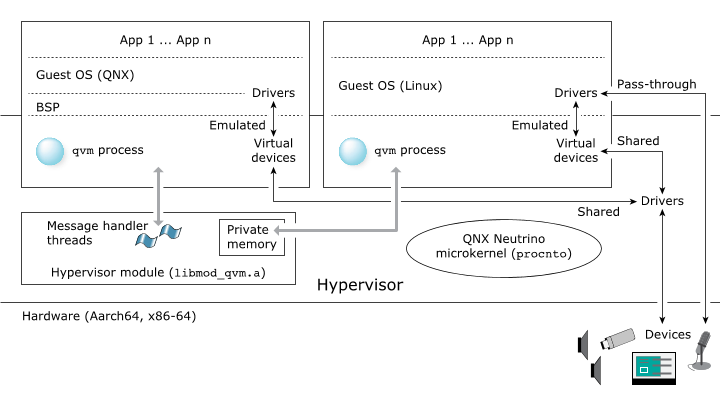
\includegraphics[width=28cm]{qvm_arch.png}\\
 \caption{Fig. 6 : QNX Architecture}
\end{center}

\end{block}


\begin{block}{References}

        \bibitem{b1}[1] Hildebrand, D.“An Architectural Overview of QNX.” USENIX Workshop on Microkernels and Other Kernel Architectures (1992).
    \bibitem{b2}[2] QNX Staff (2004-08-17). "QNX Delivers Extremely Reliable Microkernel for Massively Scalable Routing System". Retrieved 2021-03-21.
    \bibitem{b3}[3] Embedded OS, Support and Services | RTOS, Hypervisor | BlackBerry QNX : https://blackberry.qnx.com/en
    \bibitem{b4}[4] Q. N. X. Community, “Analyzing Memory Usage and Finding Errors,” QNX Momentics IDE User's Guide, 12-Dec-2012. http://www.qnx.com/developers/docs/6.5.0/index.jsp 

\end{block}



\end{column} % End of the third column

\end{columns} % End of all the columns in the poster

\end{frame} % End of the enclosing frame

\end{document}